\begin{frame}{Feature Visualization}
  \centering
  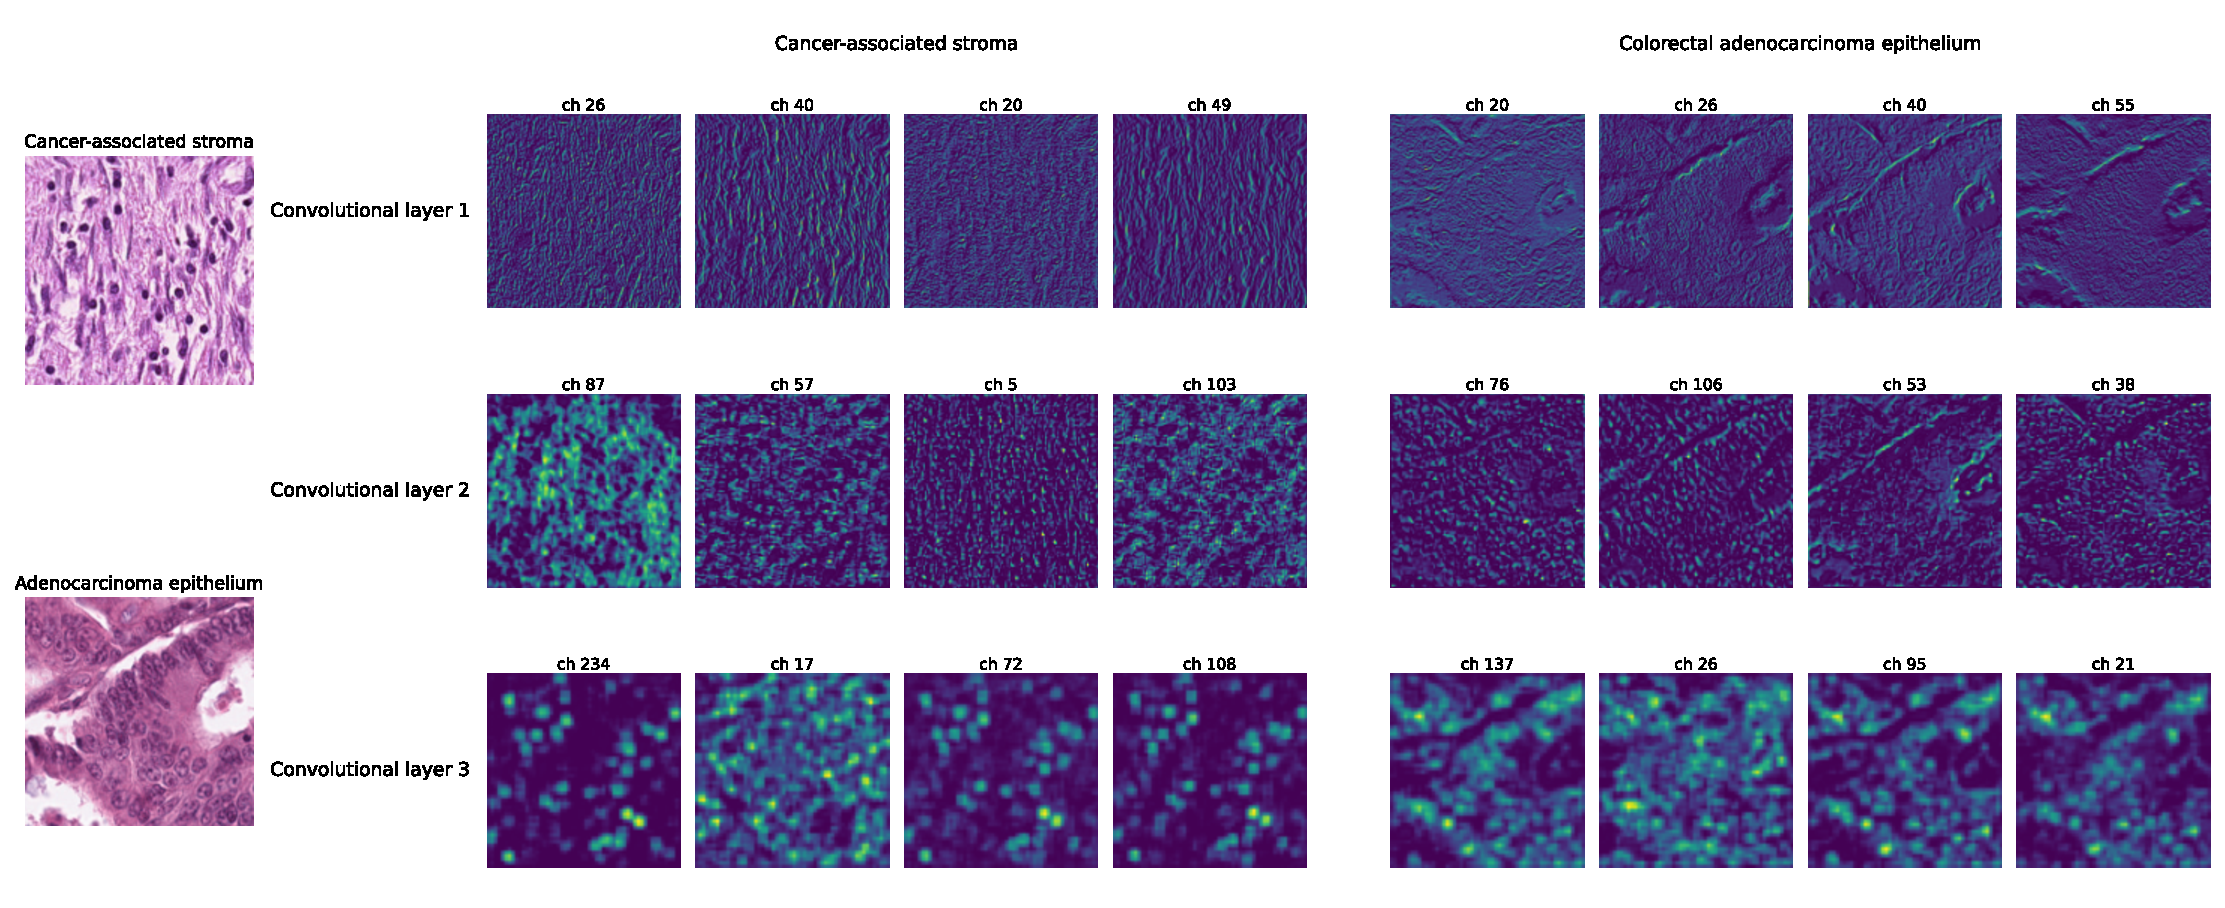
\includegraphics[width=0.90\textwidth]{figures/baseline224_cancer_feature_maps}
  \vspace{0.4em}
  \begin{itemize}
    \item Epithelium activations become more localized in deeper layers.
    \item Stroma activations stay more diffuse, suggesting a less stable representation.
  \end{itemize}
\end{frame}

\begin{frame}{Grad-CAM Visualization}
  \centering
  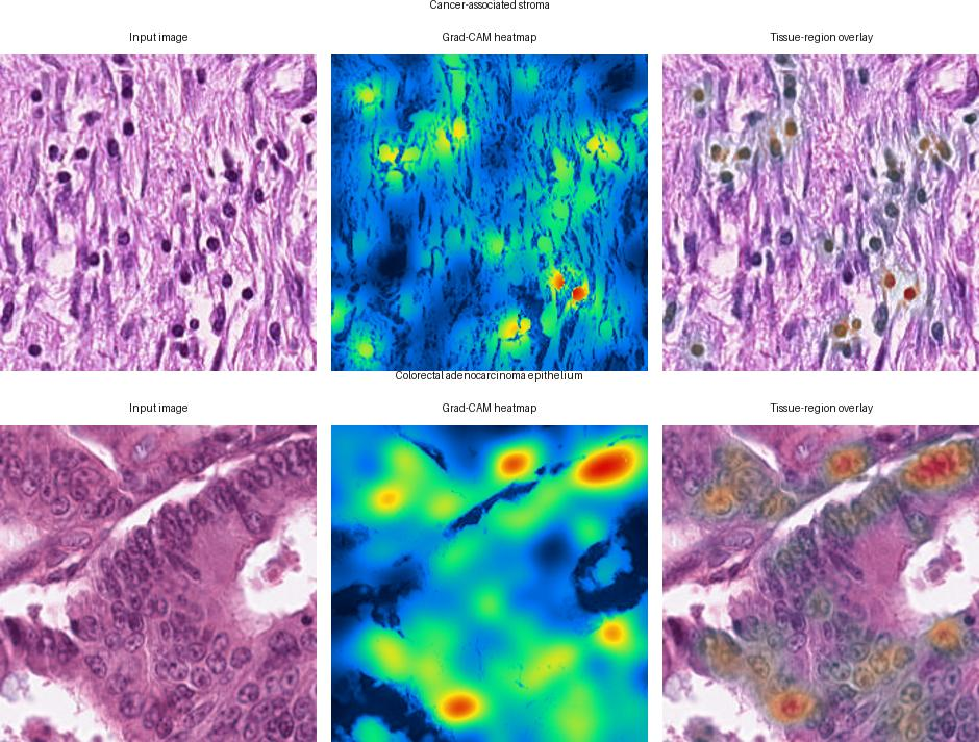
\includegraphics[height=0.86\textheight]{figures/baseline224_cancer_gradcam_vertical}
  % \begin{itemize}\small
  %   \item Stroma decisions are based on distributed texture-like regions.
  %   \item Epithelium decisions are more localized around dense epithelial structures.
  % \end{itemize}
\end{frame}

\begin{frame}{Prediction Confidences}
  \centering
  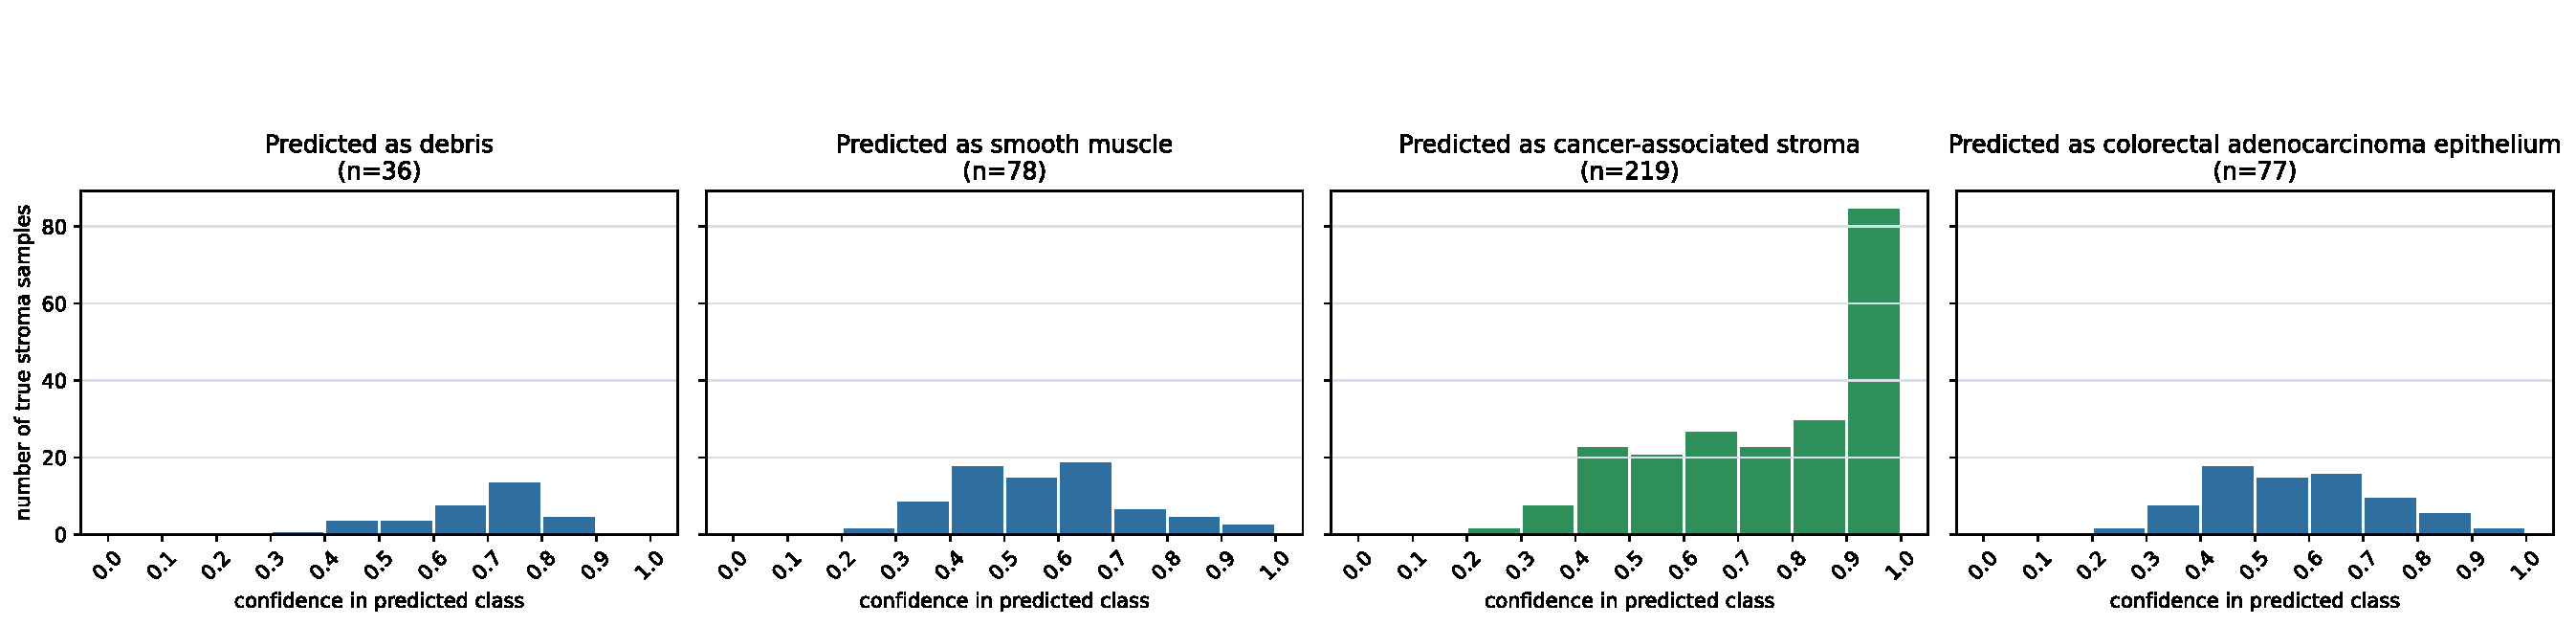
\includegraphics[width=0.94\textwidth]{figures/baseline224_stroma_confidence_distributions}
  \vspace{0.1em}
  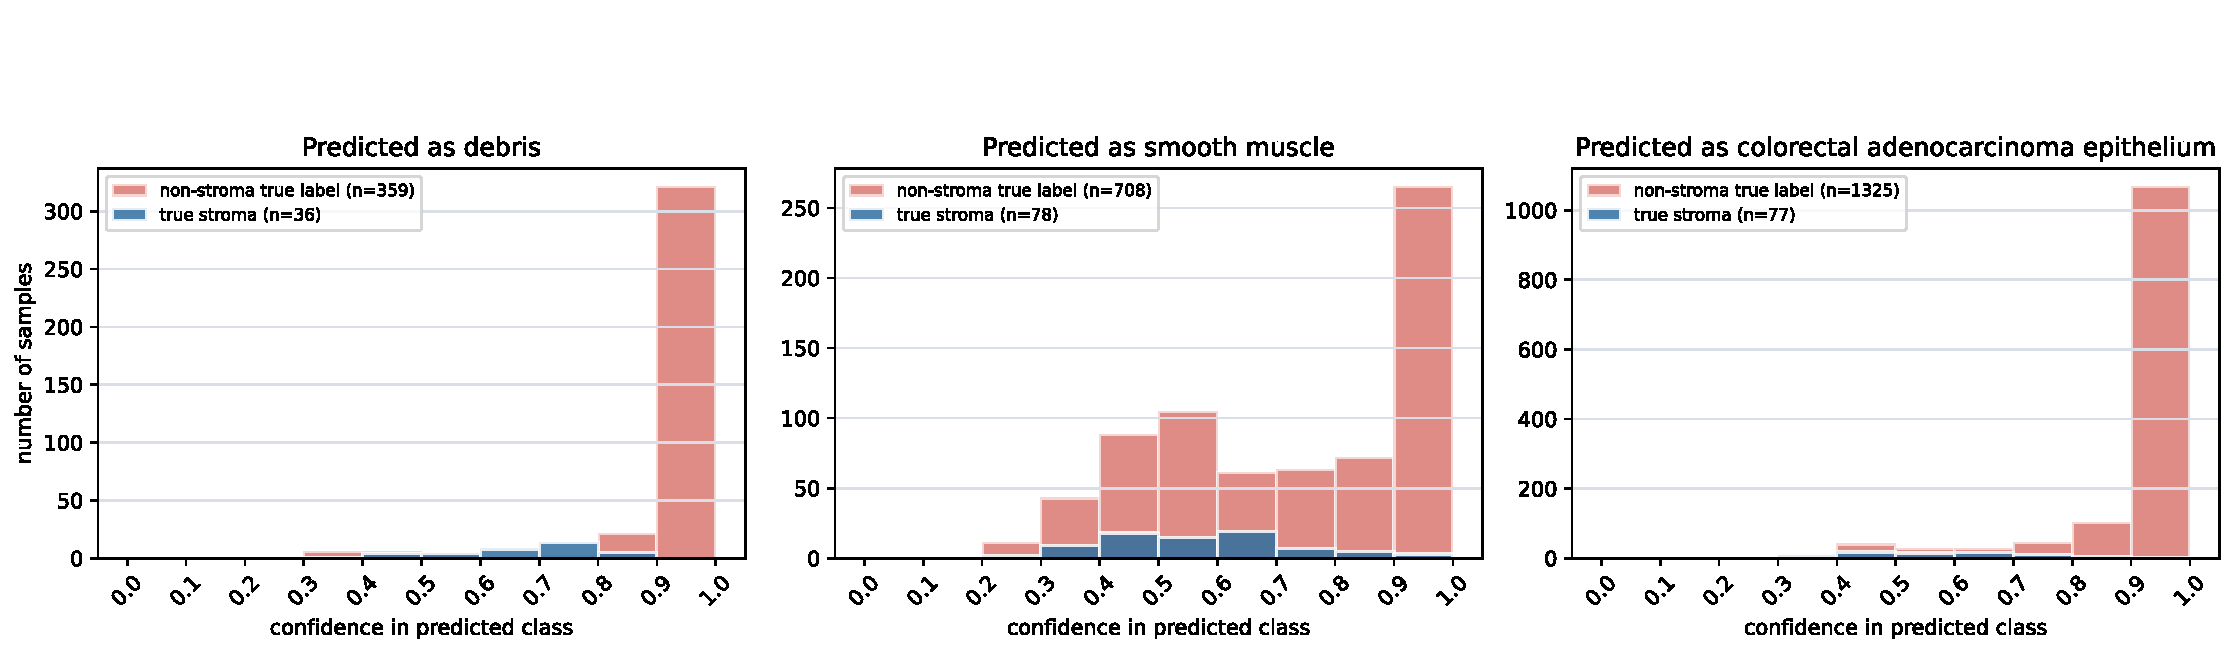
\includegraphics[width=0.94\textwidth]{figures/baseline224_stroma_nonstroma_confidence_comparison}
  % \begin{itemize}
  %   \item Many true stroma false negatives have only moderate confidence.
  %   \item High-confidence non-stroma predictions can usually be kept.
  %   \item Low-confidence predictions are candidates for specialist correction.
  % \end{itemize}
  % \begin{block}{Trigger rule}
  %   Consult an expert when the base model predicts a competing class with confidence below $\tau = 0.9$.
  % \end{block}
\end{frame}

\begin{frame}{Cancer Expert System}
  \centering
  \resizebox{0.96\textwidth}{!}{\begin{tikzpicture}[
    scale=0.7, transform shape,
    >=Latex,
    font=\small,
    box/.style={
        draw,
        rounded corners,
        thick,
        align=center,
        minimum height=1.1cm,
        minimum width=2.8cm,
        fill=blue!5
    },
    decision/.style={
        draw,
        diamond,
        thick,
        align=center,
        aspect=2.2,
        inner sep=1.2pt,
        fill=orange!8,
        text width=4.2cm
    },
    output/.style={
        draw,
        rounded corners,
        thick,
        align=center,
        minimum height=1.0cm,
        minimum width=2.1cm,
        fill=green!5
    },
    outer/.style={
        draw,
        rounded corners,
        very thick,
        inner xsep=10pt,
        inner ysep=10pt
    }
]

% --------------------------------------------------
% Nodes
% --------------------------------------------------

% Input centered between upper and lower paths
\node (input) at (-3.8,0) [box] {Sample $x$};

% Upper path
\node (base) at (0,1.4) [box, visible on=<2->] {Base model $\mathcal M_B$};
\node (baseout) at (3.0,1.4) [output, minimum width=1.3cm, visible on=<3->] {$\hat y_B$};
\node (decision) at (7.9,1.4) [decision, visible on=<4->]
{$\hat y_B \in \mathrm{Experts},$\\[2pt]
$p_B(\hat y_B \mid x) < \tau$};

\node (finalbase) at (13.3,1.4) [output, minimum width=2.3cm, visible on=<5->]
{$\hat y = \hat y_B$};

% Lower path
\node (expert) at (7.9,-1.4) [box, minimum width=2.9cm, visible on=<6->]
{Expert $\mathcal M_E$};

\node (finalexpert) at (13.3,-1.4) [output, minimum width=2.3cm, visible on=<7->]
{$\hat y = \hat y_E$};

% Final output outside the system box
\node (final) at (16.7,0) [output, minimum width=1.4cm, visible on=<8->]
{$\hat y$};

% --------------------------------------------------
% Helper coordinates
% --------------------------------------------------

\coordinate (inbranch) at (-1.8,0);
\coordinate (merge) at (14.8,0);

% --------------------------------------------------
% Arrows
% --------------------------------------------------

% Sample branching to both paths
\draw[-, thick, visible on=<2->] (input.east) -- (inbranch);
\draw[->, thick, visible on=<2->] (inbranch) |- (base.west);
\draw[->, thick, visible on=<6->] (inbranch) |- (expert.west);

% Main upper path
\draw[->, thick, visible on=<3->] (base) -- (baseout);
\draw[->, thick, visible on=<4->] (baseout) -- (decision);

% Decision branches
\draw[->, thick, visible on=<5->] (decision) -- node[above] {no} (finalbase);
\draw[->, thick, visible on=<6->] (decision) -- node[right] {yes} (expert);

% Expert output
\draw[->, thick, visible on=<7->] (expert) -- (finalexpert);

% Merge both internal outputs into final output
\draw[thick, visible on=<8->] (finalbase.east) -| (merge);
\draw[thick, visible on=<8->] (finalexpert.east) -| (merge);
\draw[->, thick, visible on=<8->] (merge) -- (final.west);

% --------------------------------------------------
% Outer system box
% --------------------------------------------------

\node[outer, fit=(base)(baseout)(decision)(expert)(finalbase)(finalexpert), visible on=<2->] (system) {};
\node[anchor=south west, font=\bfseries, visible on=<2->] at (system.north west)
{Cancer Expert};

\end{tikzpicture}
}
\end{frame}

\section{Results}
